\documentclass{article}
\usepackage{a4wide}
\usepackage{graphicx}

\begin{document}

\begin{titlepage}
    \begin{center}
        Rising Sun Pictures \\
        \vspace{1cm}
        \begin{center}                
        
\includegraphics{fig/earth.png} \\
        \end{center}
        \vspace{5cm}
        {\LARGE\bf GUI Plugins} \\
        \vspace{5cm}
        {\LARGE\bf Development Documentation} \\
        \vspace{6cm}
        \today
    \end{center}
\end{titlepage}

\tableofcontents
\listoffigures
\newpage

\section{Introduction} % (fold)

\noindent
The development of the web-based Earth application by Rising Sun Pictures (RSP) over the Ruby-On-Rails (ROR) framework further illustrates the benefits of software reuse in terms of enhancing the versatility and extensibility of software applications. Instead of building the application from the ground up, the Earth application is developed atop the base code that is auto-generated by the relevant components of the underlying ROR framework. This development strategy means that the design of the Earth application is leaning significantly towards the Model-View-Controller (MVC) template of ROR-based software applications. The other application components of the Earth application such as the daemon and the built-in web server is then designed around the auto-generated base code. Presently, having been developed with a RSP design philosophy in mind, these additional codes (around the ROR auto-generated base code) are relatively static and requires significant efforts in order to accommodate new or later requirements. 

\noindent
As part of the project, the possibility of further developing the application in order to accommodate the reconfiguration of the existing design at a later stage was investigated. Such a reconfiguration option involves compartmentalising the various aspects of the existing web-based Graphical User Interface (GUI). A further goal of this initiative is to simplify the process with which the users of the Earth application could reconfigure the current GUI according to their own designs or requirements specifications. This exploratory task uncovered the ROR provisions for the plugin-type reconfiguration of the base code. 

\noindent
The following section will present how the existing ROR plugin provisions are activated and included as part of the reconfiguration option for the web-based Earth application.

% (end)

\section{Development Updates} % (fold)

\noindent
The actual implementation of the GUI plugin was reached through a number of exploratory and discovery stages namely, the investigation of the existing plugin provisions in the ROR framework, the preparation by design of the demarcated features and functionalities, and the actual implementation in code of the approved GUI plugin design. 

\subsection{Investigation} % (fold)

\noindent
Upon closer examination, it was established that the ROR plugin provisions can effectively enable the implementation of independent functional modules for the Earth application web-based GUI. This revelation means that there is no real need to devise or create an entirely different plugin manager for the GUI plugins as the existing ROR framework has adequate facility for such feature. However, since the various component for each GUI would have to be placed in different parts of the code in conformance to the MVC design aesthetics, figuring out each parts and where it should be placed imposes some challenges for the user or developed tasked with creating the GUI plugins. Nevertheless, the ROR framework provides a neat way of dealing with challenge and simplifies the development process a great deal still. 

\noindent
A ROR plugin is either an extension or a modification of the core framework. Such plugins can do almost anything that a ROR application can. The provided plugin generator script is able to copy the respective files into their respective application sub-directories. In addition, the generator script can process an ERB file and have it copied into the migration folder through the use of the following migration templates: 

\begin{itemize}
    \item{\textbf{Models}} Put a model in the plugin’s \texttt{lib} folder and use \texttt{generator} to copy it to \texttt{app/models} folder.
    \item{\textbf{View Helpers}} A helper method can be included, or mixed, into the rest of the application. (This is also known as ``mixin''.) 
    \item{\textbf{Controllers}} Copies a controller into the \texttt{app/controllers} directory. 
    \item{\textbf{rake Tasks}} Creates a \texttt{rake} file into the tasks folder.
    \item{\textbf{Images, Stylesheets, Javascripts}} The \texttt{generator} copies these into the public directory.
    \item{\textbf{Test assertions}} To be mixed-in to the tests cases.
    \item{\textbf{Unit and Functional tests}} Can be generated like controllers.
\end{itemize}

Ultimately, this investigative process confirmed that the ROR plugin framework can be used to create GUI plugins for the Earth application project.

% (end)

\subsection{Preparation} % (fold)

Creating a GUI plugin using the ROR framework requires the satisfactory completion of a number of preparatory tasks. First, a clear description and conceptual design of the proposed plugin-able feature should be documented and determined as being logically sound. All aspects of this proposed feature should be then be identified such as the relevant source files that needs to be created or modified. Information about where these files will reside within the codebase should also be established before the relevant generator script, which will process and copy the files into the app subdirectory of Earth application codebase, is invoked. A detailed description of the actual implementation in code is provided next.

% (end)

% (end)

\section{Implementation} % (fold)

The GUI plugins are implemented using the ROR plugin framework. However, some code changes had to be made to the original `VIEW' codes. This is to allow the seamless addition of extra features such as a new tag or search field. The structure of the ROR plugin framework is shown in Figure \ref{fig:flow} below.

\begin{figure}[ht]
    \centering
    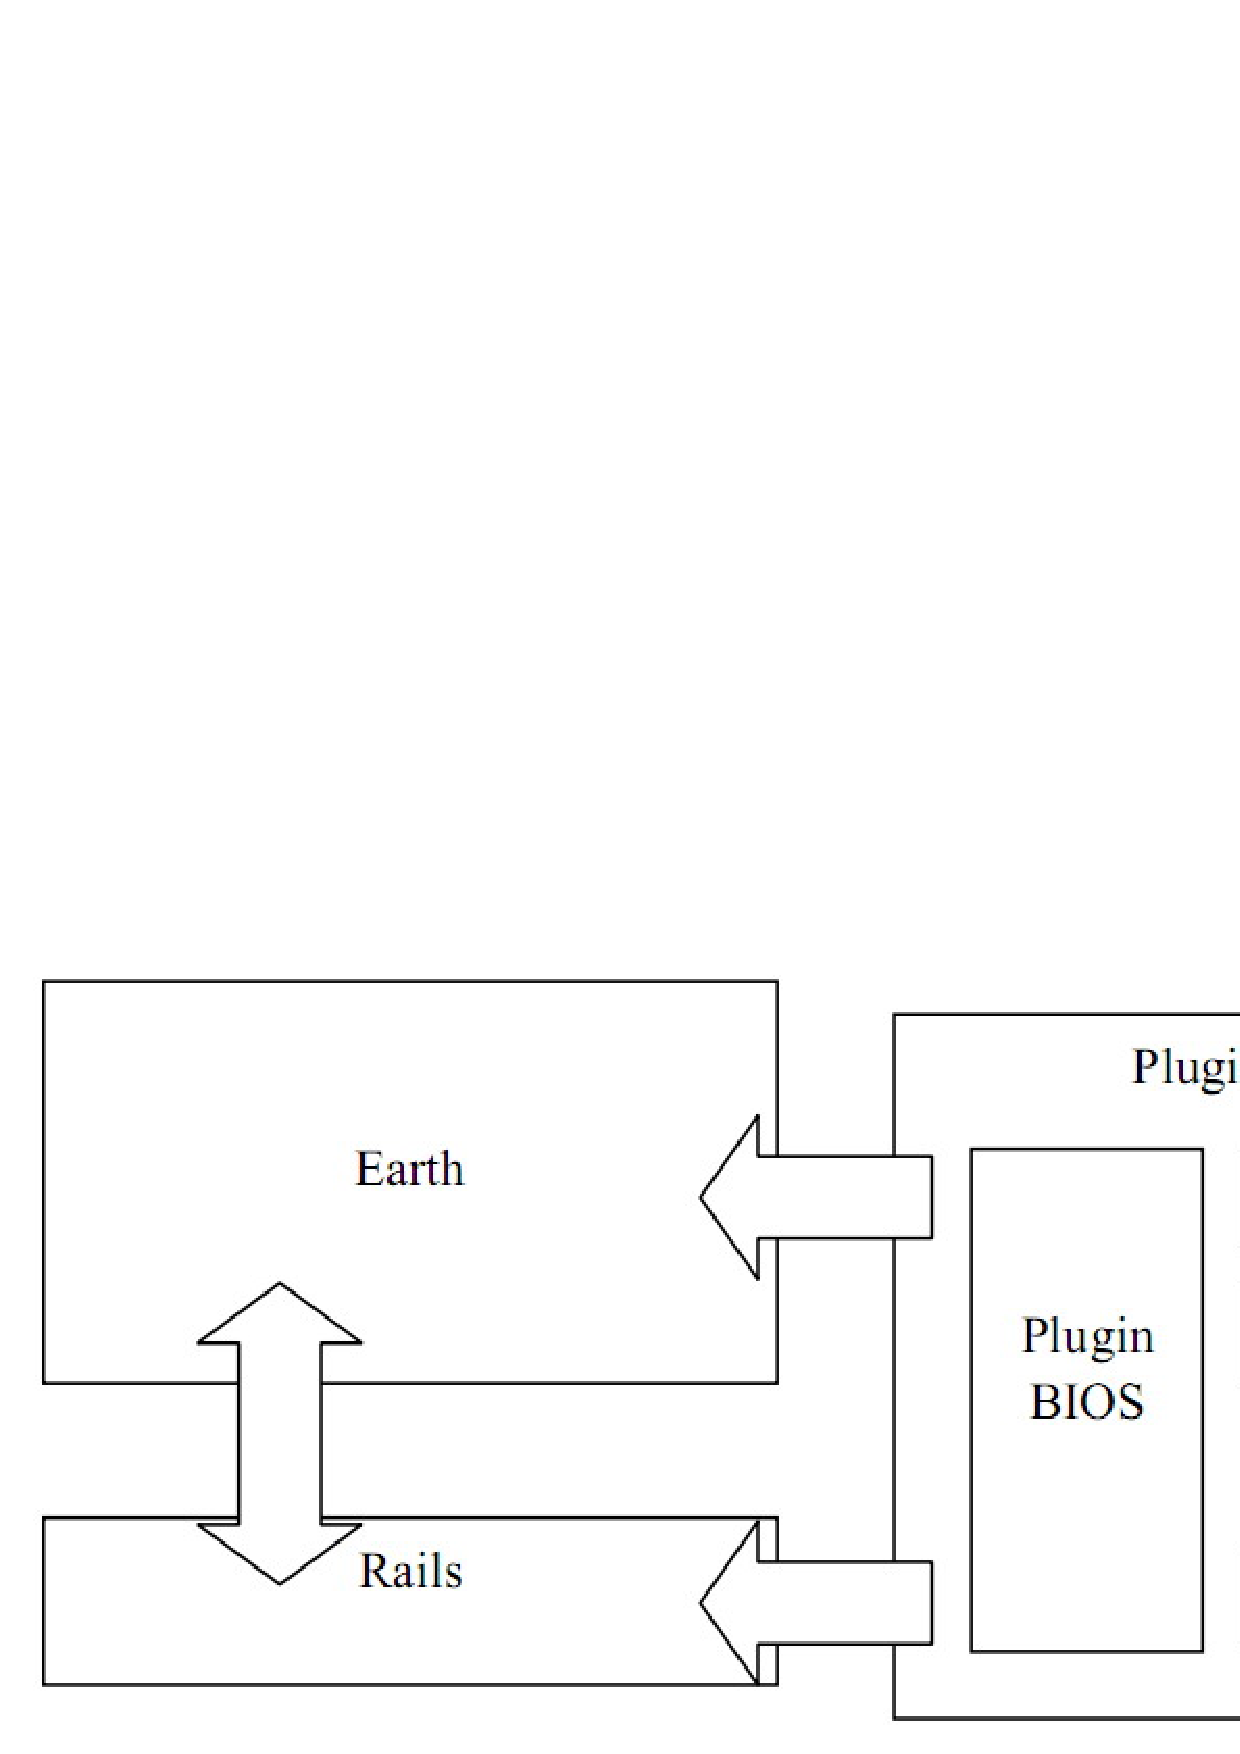
\includegraphics[scale=0.4]{fig/flow.png}
    \caption{The structure of the GUI Plugin framework.}
    \label{fig:flow}
\end{figure}

The ROR plugin framework is being adopted to extend the existing features and functionality of the Earth application. This resulted in the creation of an intermediate conceptul layer that is designed to facilitate the communication between the plugins, the Earth application daemon and the codes of the underlying ROR framework. This conceptual layer can be further expanded to include dependency checks and sub-classing feature. This also means that for each plugin, the configuration file `plugin.cfg' is created for the purpose of retaining information about the corresponding plugin. This configuration file is then used as a manifest of the plugin package.

% (end)

\section{Instruction} % (fold)

This section will describe the steps on how to develop, install and uninstall a GUI plugin for the Earth application. For ease of explanation, a simple yet fully-featured plugin called `mr\_bogus' is used as an example. Figure \ref{fig:instruction-1} shows a screenshot of the web-based GUI for the Earth application before the `mr\_bogus' plugin is installed.

\begin{figure}
    \centering
    
\includegraphics[scale=0.5]{fig/instruction-1.jpg}
    \caption{Original Earth front-end.}
    \label{fig:instruction-1}
\end{figure}

\subsection{Development} % (fold)

As mentioned before, the generate script is first executed to create some basic necessary structures and files. To do so, the following command can be used:

\begin{verbatim}
    ./script/generate plugin mr_bogus --with generator
\end{verbatim}

\begin{figure}
    \centering
    
\includegraphics[scale=0.5]{fig/instruction-2.jpg}
    \caption{Running the \texttt{generate} script to create mr\_bogus plugin.}
    \label{fig:instruction-2}
\end{figure}

A blank plugin in Rails have been created after the previous command was executed successfully. At this stage, one can safely edit the affected files to have the final results displayed. Views can be added by creating new directories and files in the \texttt{./vendor/plugins/mr\_bogus/generators/ mr\_bogus/templates} directory. For example, the action controller needs the directory called ``controllers''. Finally, update the file called ``mr\_bogus\_generator.rb'', which can be executed to create particular file wherever one wants. More instructions can be found in this web-site \texttt{http://wiki.rubyonrails.com/rails/pages/HowTosPlugins}.

Here an action controller and a webpage were created for views:

\begin{verbatim}
./vendor/plugins/mr_bogus/generators/mr_bogus/templates/controllers/bogus_controller.rb
./vendor/plugins/mr_bogus/generators/mr_bogus/templates/views/bogus.rhtml
\end{verbatim}

Figure \ref{fig:instruction-3} shows the content of the \texttt{bogus\_controller.rb} file, and Figure \ref{fig:instruction-4} shows the content of the \texttt{bogus.rhtml} file.

\begin{figure}
    \centering    
    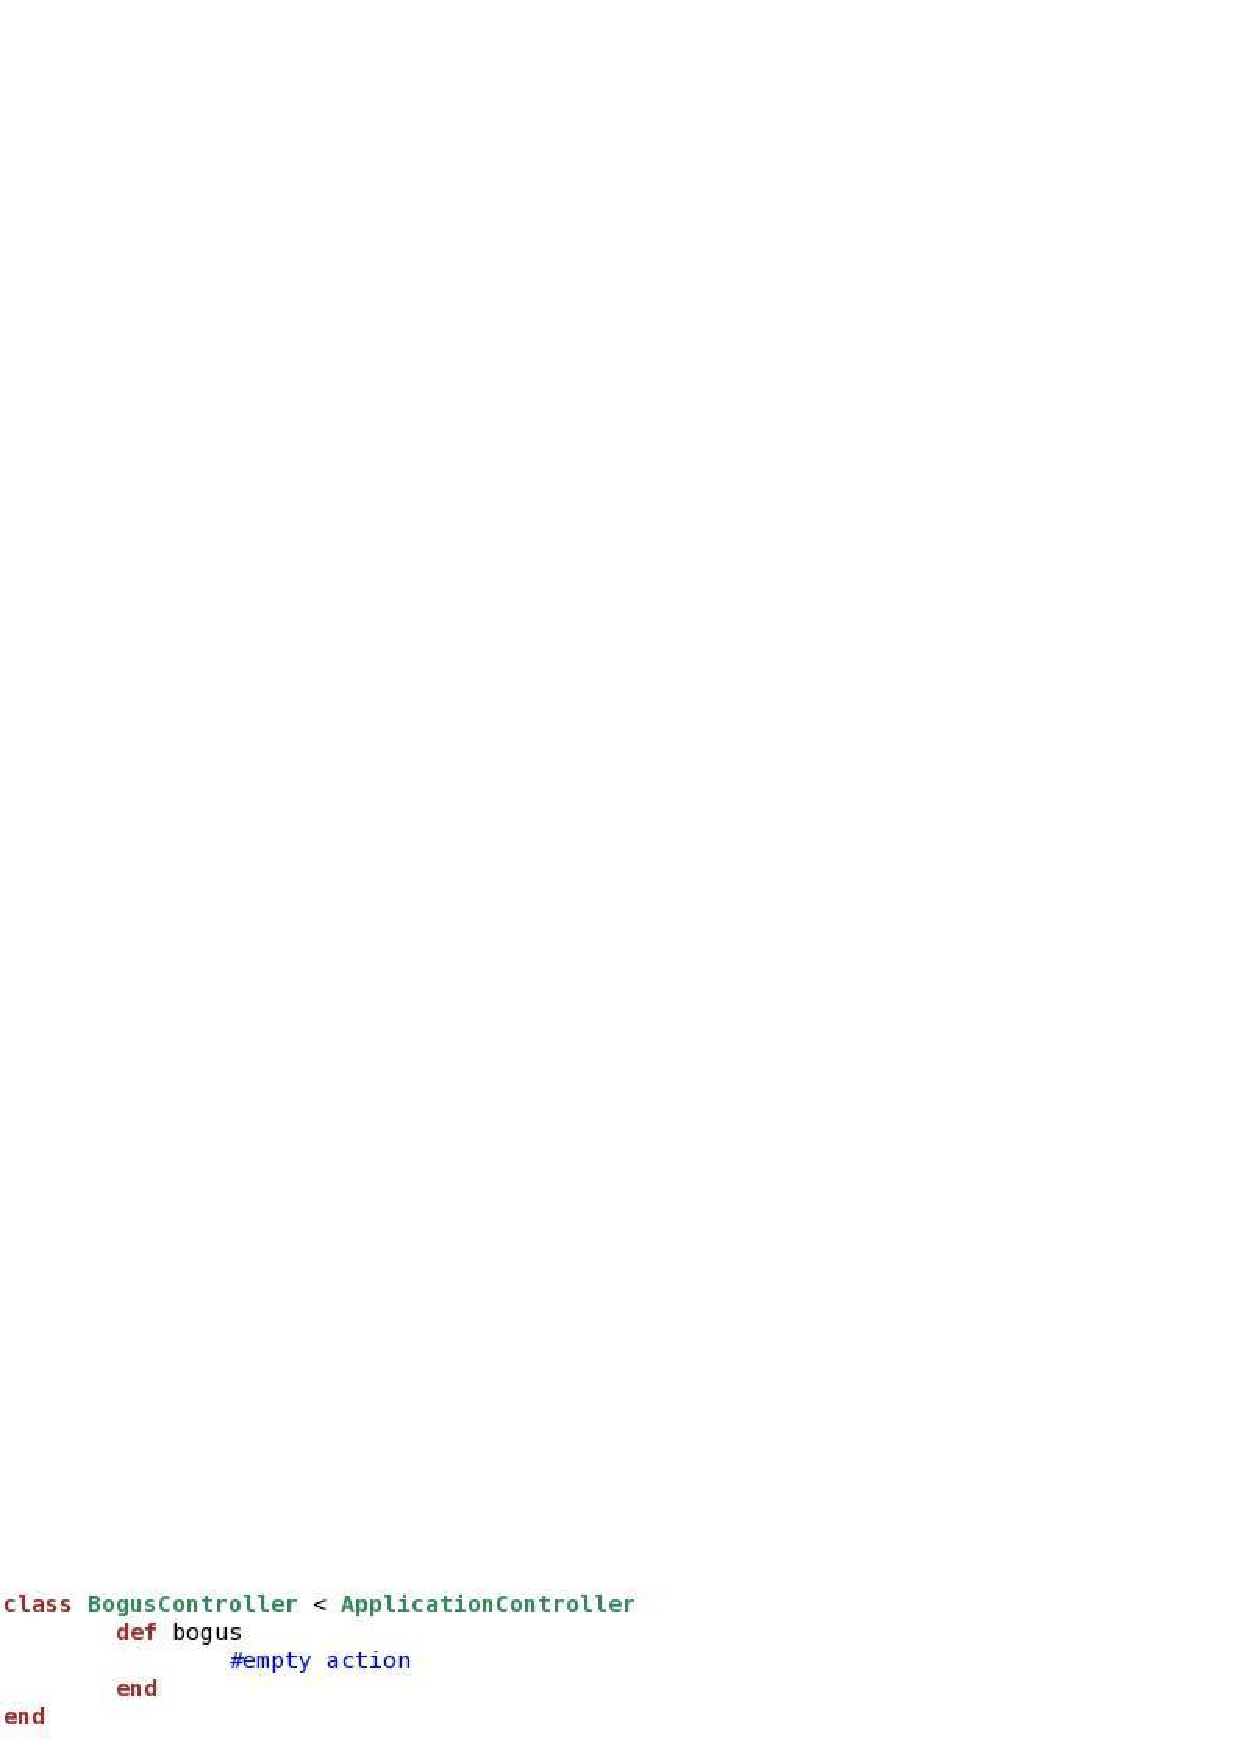
\includegraphics[scale=0.5]{fig/instruction-3.jpg}
    \caption{The \texttt{bogus\_controller.rb} file.}
    \label{fig:instruction-3}
\end{figure}

\begin{figure}
    \centering
    
\includegraphics[scale=0.5]{fig/instruction-4.jpg}
    \caption{The \texttt{bogus.rhtml} file.}
    \label{fig:instruction-4}
\end{figure}

The file named \texttt{mr\_bogus\_generator.rb} would be modified for preparation of moving files to particular folders, as shown in Figure \ref{fig:instruction-5}.

\begin{figure}
    \centering    
    
\includegraphics[scale=0.5]{fig/instruction-5.jpg}
    \caption{The \texttt{mr\_bogus\_generator.rb} file.}
    \label{fig:instruction-5}
\end{figure}

Once done, the following command can be executed to have the plugin implemented into Rails: 

\begin{verbatim}
./script/generator mr_bogus bogus
\end{verbatim}

To test the plugin, simply point the web-browser of choice to the following URL:

\begin{verbatim}
http://localhost:3000/bogus/bogus
\end{verbatim}

However, the plugin should be implemented into the existing Earth system instead. To do so, a configuration file has to be created. The file is named ``plugin\_cfg'' in the \texttt{./vendor/plugins/mr\_bogus} directory. Figure \ref{fig:asd} shows the content of the configuration file.

\begin{figure}
    \centering
    
\includegraphics[scale=0.5]{fig/asd.jpg}
    \caption{The \texttt{plugin\_cfg} file.}
    \label{fig:asd}
\end{figure}

Now, point the web-browser to the homepage of Earth. The result is shown in Figure \ref{fig:instruction-6}. Figure \ref{fig:instruction-7} shows the implementation of the plugin.

\begin{figure}
    \centering        
    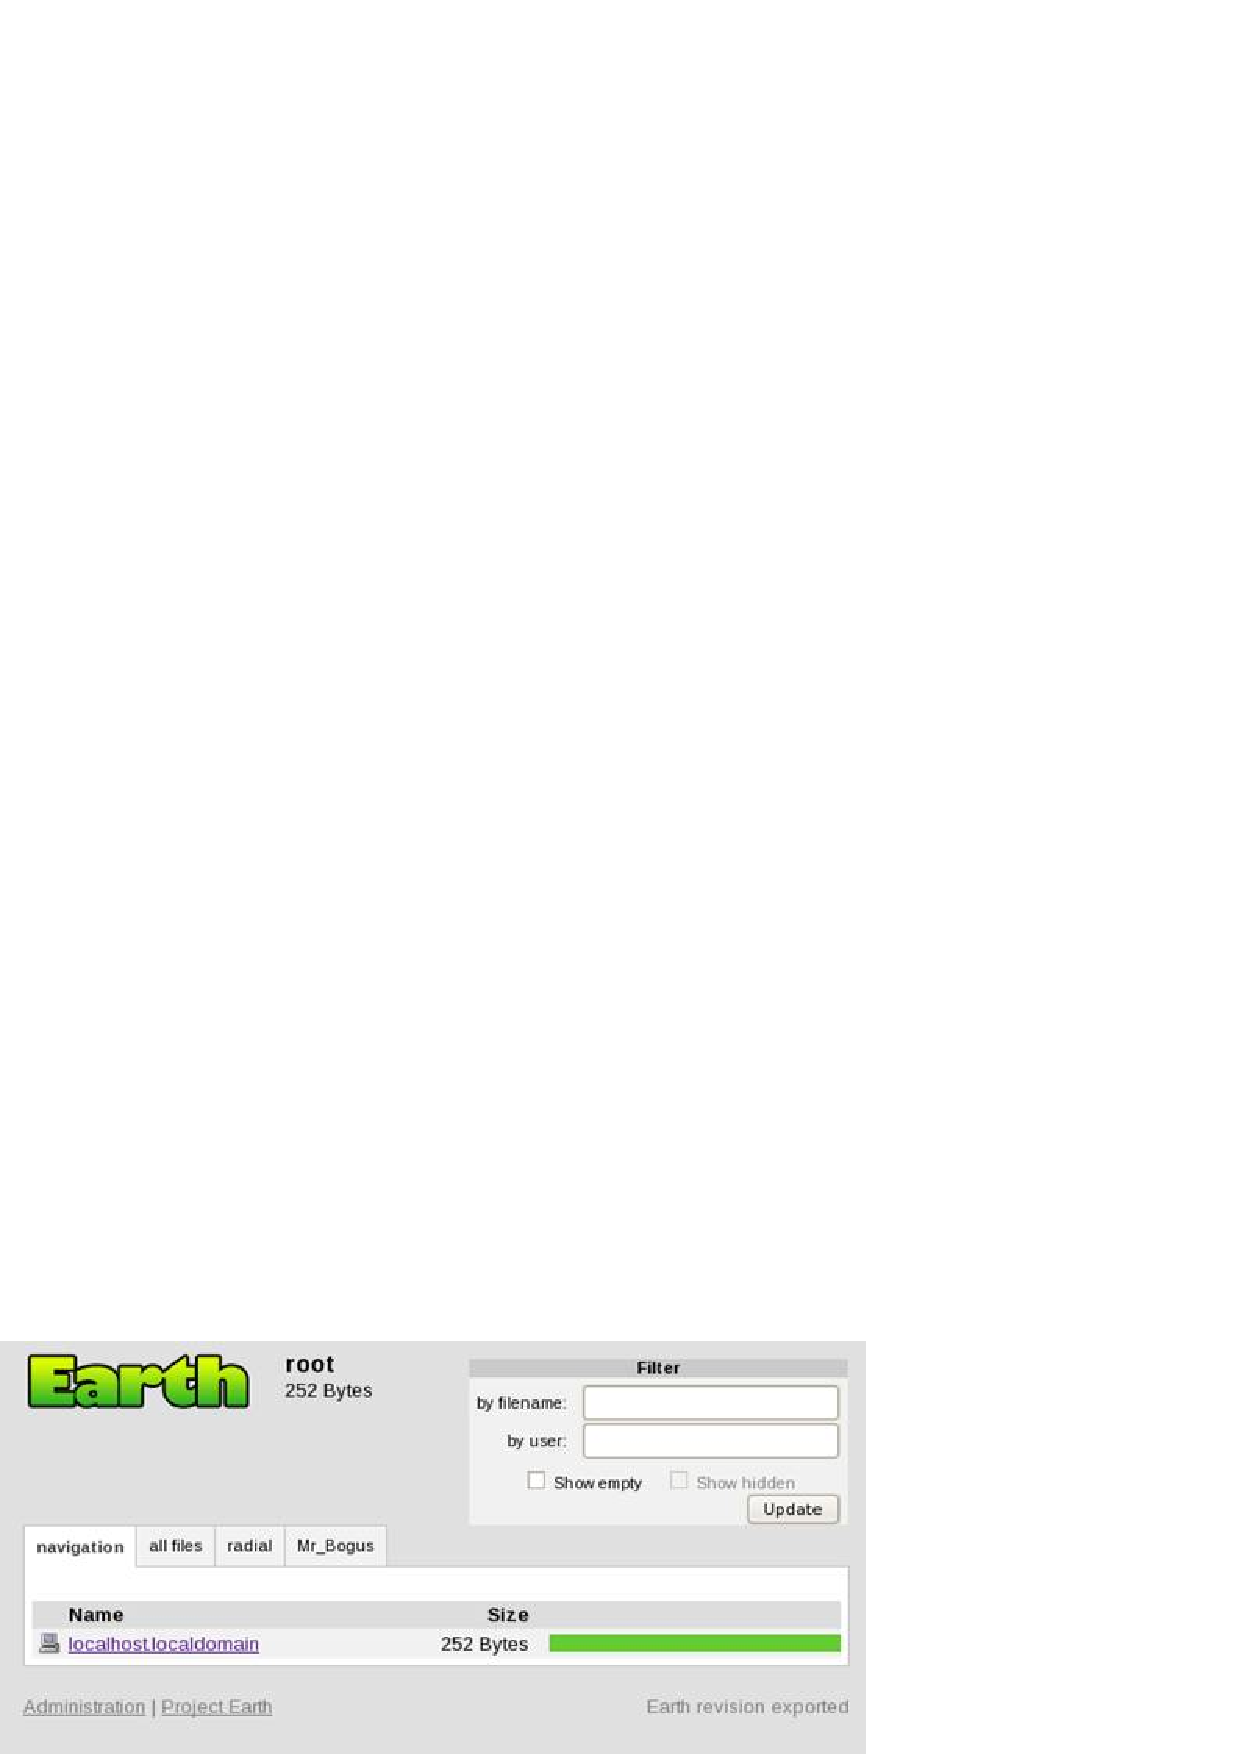
\includegraphics[scale=0.5]{fig/instruction-6.jpg}
    \caption{\texttt{mr\_bogus} implemented in Earth.}
    \label{fig:instruction-6}
\end{figure}

\begin{figure}
\centering

\includegraphics[scale=0.5]{fig/instruction-7.jpg}
\caption{The \texttt{mr\_bogus} tab.}
\label{fig:instruction-7}
\end{figure}

So far, the plugin had included a new tab in Earth. However, to add a new text field in the filter section, the following can statements can be added into the configuration file:

\begin{verbatim}
    #require componenet, view string, parameter name
    field_tag, by wine, wine
    field_tag, by cake, cake
\end{verbatim}

Figure \ref{fig:instruction-9} shows the refreshed the homepage of Earth.

\begin{figure}
    \centering
    
\includegraphics[scale=0.5]{fig/instruction-9.jpg}
    \caption{New text fields.}
    \label{fig:instruction-9}
\end{figure}

The plugin can now be tested and debugged. Finally, a set of installation and uninstallation scripts can be created from the following steps:

\begin{enumerate}
    \item Find files and folders created.
    \item Modify the installation in root of plugin to have the appropriate files copied to their appropriate destination directories.
    \item Build the plugin as a package including the installation file.
\end{enumerate}

The following is the content of installation of ``mr\_bogus'' named ``install.rb'':

\begin{verbatim}
    require 'fileutils' 
    plugin_name = ARGV[1] # mr_bogus 
    earth_root = ARGV[0]  
    puts "Creating the plugin" 
    system "ruby #{earth_root}/script/generate plugin #{plugin_name} --with-generator" 
    RAILS_ROOT = earth_root 
    FileUtils.cp File.join(File.dirname(__FILE__), 'init.rb'),File.join
    (RAILS_ROOT, 'vendor','plugins',plugin_name,'init.rb')  
    FileUtils.cp File.join(File.dirname(__FILE__), 'install.rb'),File.join
    (RAILS_ROOT, 'vendor','plugins',plugin_name,'install.rb')  
    FileUtils.cp File.join(File.dirname(__FILE__), 'uninstall.rb'),File.join
    (RAILS_ROOT, 'vendor','plugins',plugin_name,'uninstall.rb')  
    FileUtils.cp File.join(File.dirname(__FILE__), 'plugin_cfg'),File.join
    (RAILS_ROOT, 'vendor','plugins',plugin_name,'plugin_cfg') 
    FileUtils.cp File.join(File.dirname(__FILE__),'lib','mr_bogus.rb'),File.join
    (RAILS_ROOT, 'vendor','plugins',plugin_name,'lib','mr_bogus.rb')  
    FileUtils.cp File.join(File.dirname(__FILE__),'generators',plugin_name,
    'mr_bogus_generator.rb'),File.join(RAILS_ROOT,'vendor','plugins',plugin_name,
    'generators',plugin_name,'mr_bogus_generator.rb')  
    Dir.mkdir("#{RAILS_ROOT}/vendor/plugins/mr_bogus/generators/mr_bogus
    /templates/controllers") unless File.directory?("#{RAILS_ROOT}/vendor/plugins
    /mr_bogus/generators/mr_bogus/templates/controllers") 
    Dir.mkdir("#{RAILS_ROOT}/vendor/plugins/mr_bogus/generators/mr_bogus
    /templates/views") unless File.directory?("#{RAILS_ROOT}/vendor/plugins/mr_bogus/generators
    /mr_bogus/templates/views") 
    FileUtils.cp File.join(File.dirname(__FILE__),'generators',plugin_name,'templates',
    'controllers','bogus_controller.rb'),File.join(RAILS\_ROOT,'vendor','plugins',
    plugin_name,'generators',plugin_name,'templates','controllers','bogus_controller.rb') 
    FileUtils.cp File.join(File.dirname(__FILE__),'generators',plugin_name,'templates','views',
    'bogus.rhtml'),File.join(RAILS_ROOT,'vendor','plugins',plugin_name,'generators',
    plugin_name,'templates','views','bogus.rhtml') 
\end{verbatim}

\noindent 
An uninstallation file named ``uninstall.rb'' for removing the plugin created. Here is an example:

\begin{verbatim}
    require 'fileutils' 
    plugin_name = ARGV[1] #mr_bogus 
    earth_root = ARGV[0]  
    puts "Uninstalling the generator" 
    system "ruby #{earth_root}/script/destroy #{plugin_name} #{plugin_name}" 
    puts "Uninstalling the plugin" 
    system "ruby #{earth_root}/script/destroy plugin #{plugin_name} --with-generator" 
    system "rm -r #{earth_root}/vendor/plugins/#{plugin_name}"
\end{verbatim}

% (end)

\subsection{Installation} % (fold)

\noindent
To install and activate the plugin, simply execute the following commands: 

\begin{verbatim}
    ruby install.rb <root_earth> <plugin_name>
    ruby <root_earth>/script/generate <plugin_name> <plugin_name>
\end{verbatim}

% (end)

\subsection{Uninstallation} % (fold)

To uninstall, execute the following command:

\begin{verbatim}
    ruby uninstall.rb <root_earth> <plugin_name>
\end{verbatim}

% (end)

% (end)

\end{document}
